\section{Results and discussion}

% Target ~15-20 pages (largest section -- this is where your contribution lives).
% Mirror Part A / Part B. Interpret results; link back to the gaps and objectives.

\subsection{Part A: Simulation results}
\label{sec:results-a}

\subsubsection{Perception envelope}

The filter's accuracy is governed by range through the $\alpha r^2/s$
measurement noise model. With the vehicle stationary 5~m from the dock the
fused noise floor is approximately 0.11~m and the filter reports
\textsc{degraded} throughout; at 2.2~m the floor drops to approximately
0.02~m, the filter is \textsc{healthy} for 92\% of the run (median position
standard deviation 0.018~m), and the velocity state tracks the true dock
velocity with amplitude ratio 0.85 and correlation 0.89
(Figure~\ref{fig:vel-check}). At the opposite extreme, marker visibility
collapses at contact range: binning fine-alignment health by ground-truth
range shows 84\% to 100\% healthy beyond 5~cm of the entry but only 21\%
inside it, a blackout produced by the large markers overflowing the camera
field of view. This measured envelope, reliable from roughly 2.5~m down to
0.05~m, motivates both the 0.10~m seat criterion and the delegation of the
final centimetres to mechanical capture.

\begin{figure}[H]
    \centering
    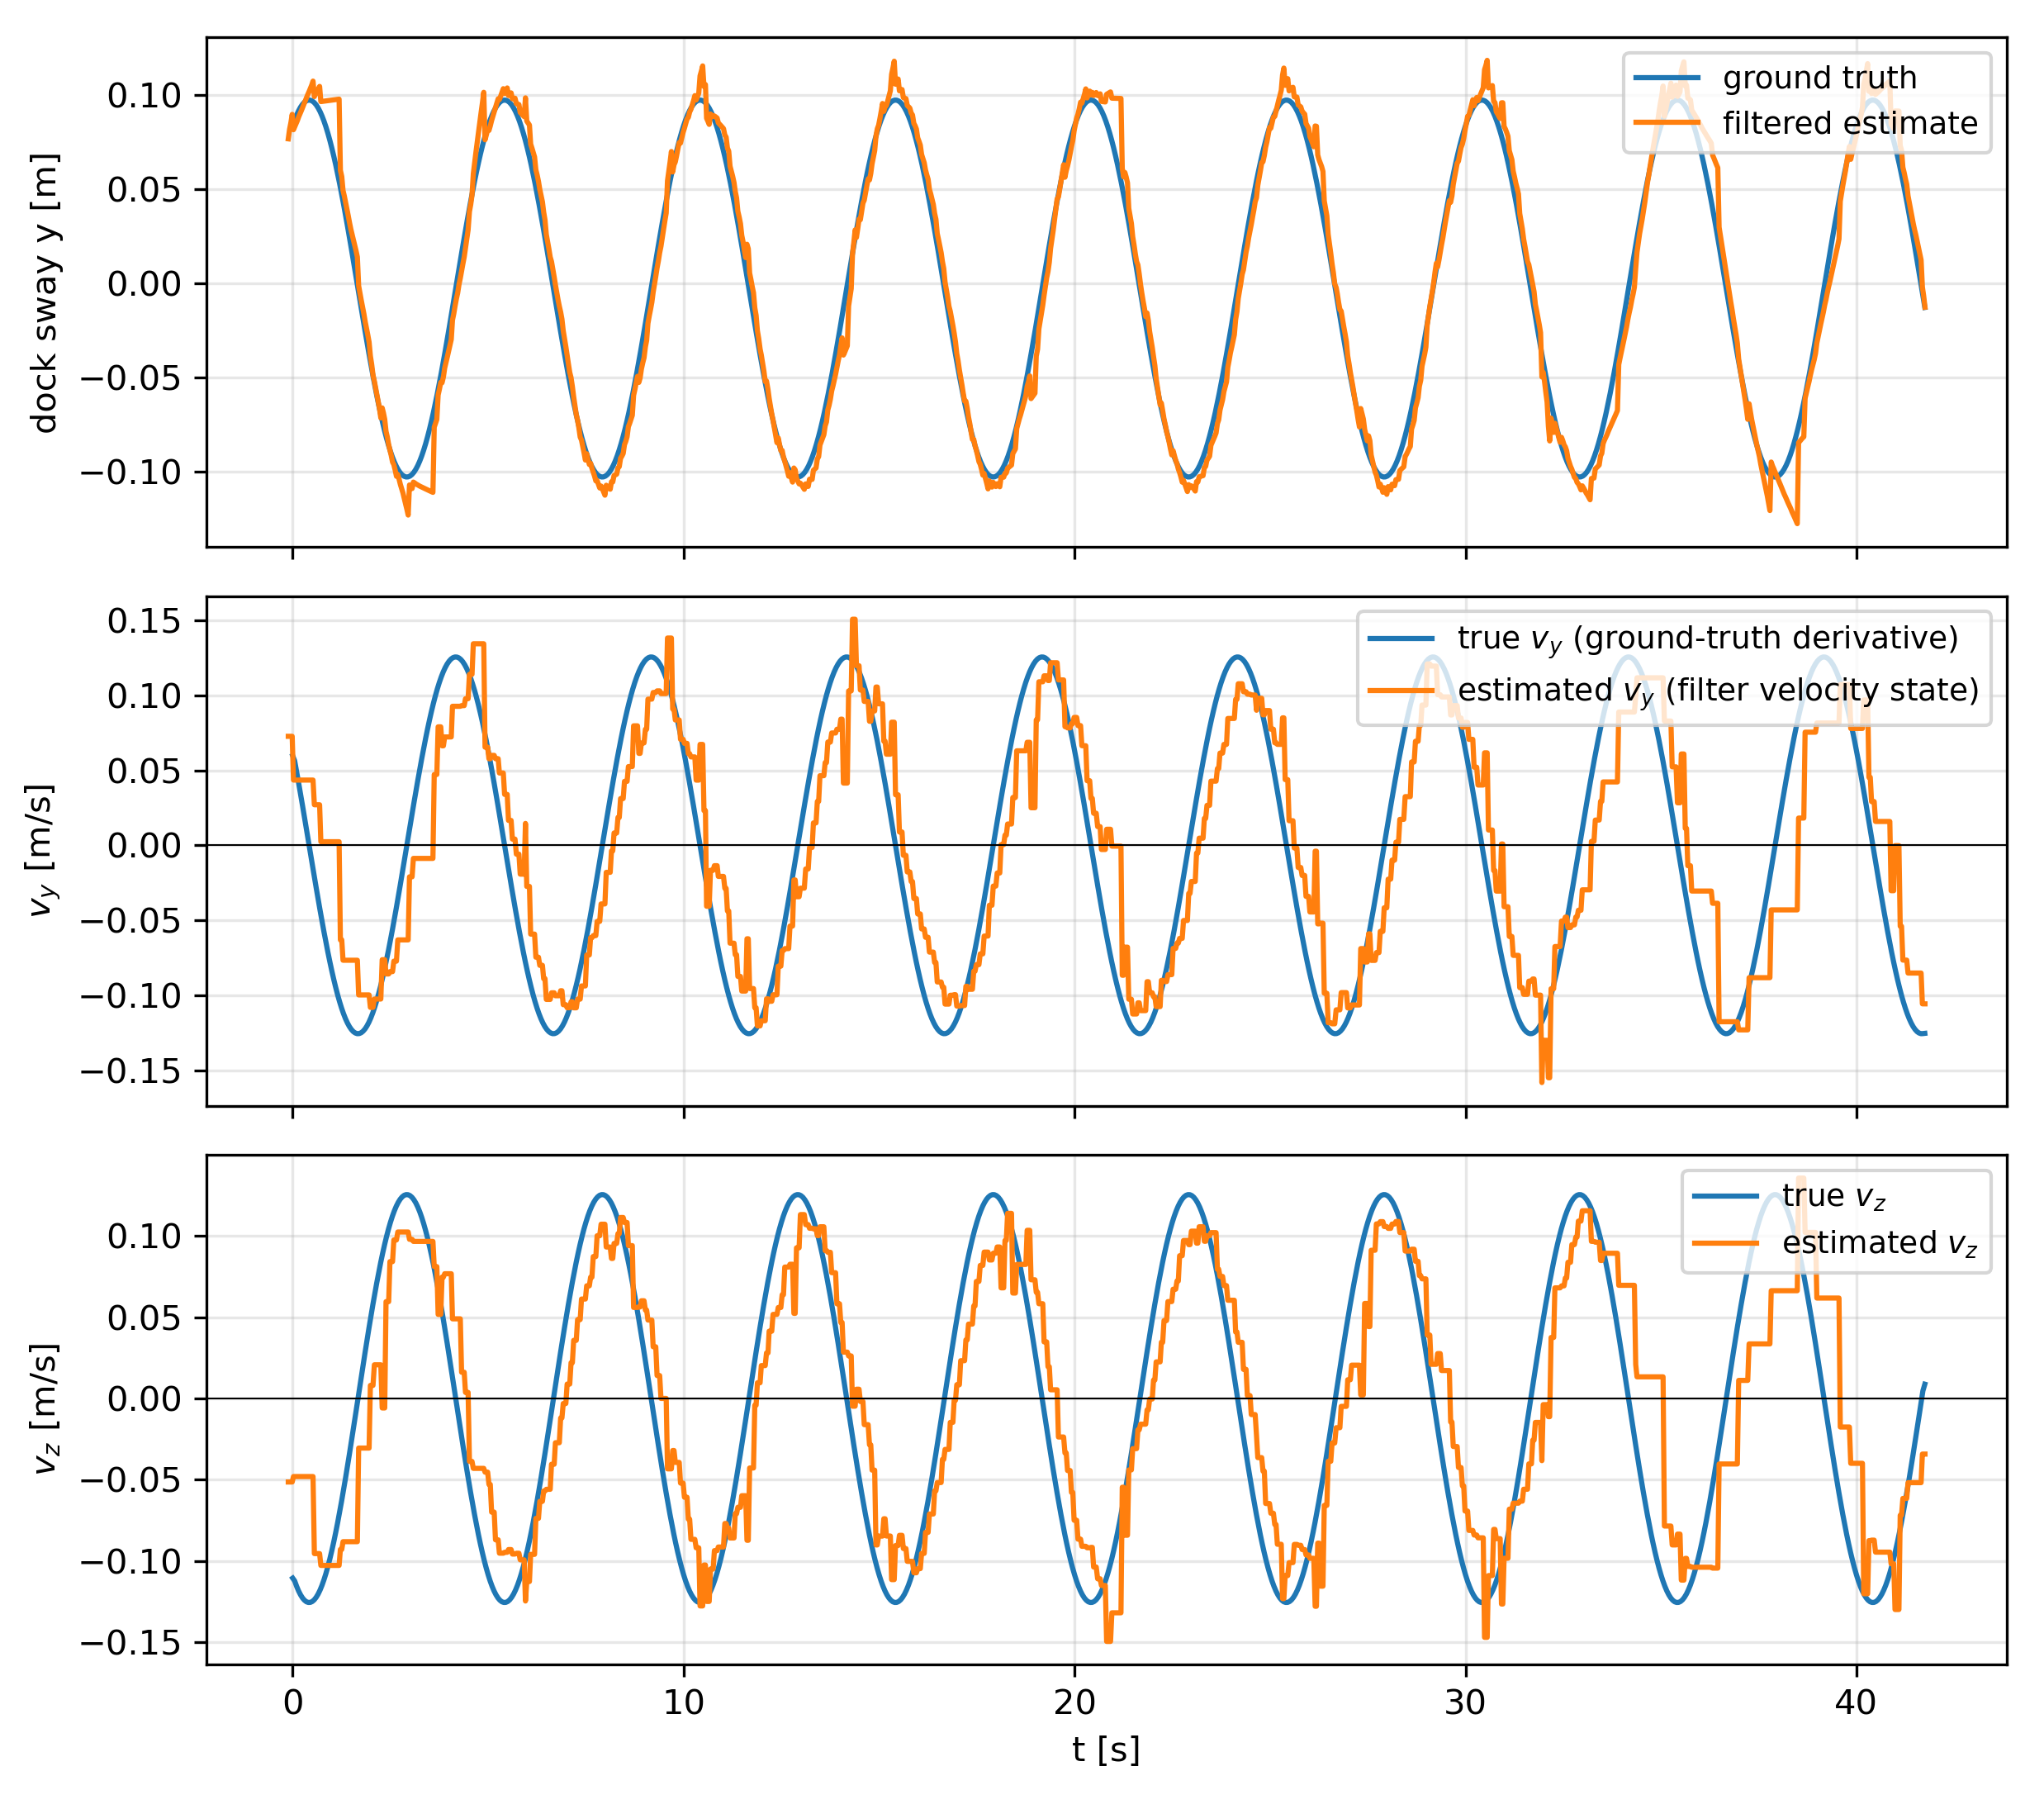
\includegraphics[width=0.85\textwidth]{Figures/vel_check.png}
    \caption{Dock velocity estimation with the vehicle stationary at 2.3~m
    (18~s sway). The velocity state (orange) tracks the ground-truth dock
    velocity (blue) at 0.85 amplitude with correlation 0.89.}
    \label{fig:vel-check}
\end{figure}

\subsubsection{Docking demonstration}

Against the nominal 18~s, 0.1~m orbital sway, the system docks
autonomously end to end: engagement to coarse at $t{+}3$~s, handoff to
fine alignment at $t{+}14$~s, seated and docked at $t{+}25$~s with no
demotions, latching 7 to 8~cm from the entry and coming to rest 4~cm in
front of the dock plane. This trial, and every sweep trial below, ran the
full perception pipeline in the loop with no ground-truth input to the
vehicle.

\subsubsection{Docking envelope versus sway period}

Table~\ref{tab:envelope} and Figure~\ref{fig:pdock} give the headline
result of the sweep ($n{=}3$ per cell, contact-censored scoring). The
baseline (static filter, no feedforward) docks in every trial at every
period in the raw scoring, and cleanly down to 8~s; at 6~s, two of three
trials brush the aperture boundary at low speed (0.03 to 0.06~m/s) before
latching. The method (constant-velocity filter with feedforward) matches
the baseline down to 12~s, degrades at 10~s (one pre-latch contact), and
fails at 8~s and 6~s; its single raw success at 8~s was contact-assisted.

\begin{table}[H]
\centering
\caption{P(dock) by sway period and scoring, $n{=}3$ per cell. Clean
excludes trials with a pre-latch off-aperture crossing.}
\label{tab:envelope}
\begin{tabular}{c|cc|cc}
 & \multicolumn{2}{c|}{Baseline (ff off)} & \multicolumn{2}{c}{Method (CV + ff)} \\
Period [s] & raw & clean & raw & clean \\
\hline
20 & 1.00 & 1.00 & 1.00 & 1.00 \\
16 & 1.00 & 1.00 & 1.00 & 1.00 \\
12 & 1.00 & 1.00 & 1.00 & 1.00 \\
10 & 1.00 & 1.00 & 1.00 & 0.67 \\
8  & 1.00 & 1.00 & 0.33 & 0.00 \\
6  & 1.00 & 0.33 & 0.00 & 0.00 \\
\end{tabular}
\end{table}

\begin{figure}[H]
    \centering
    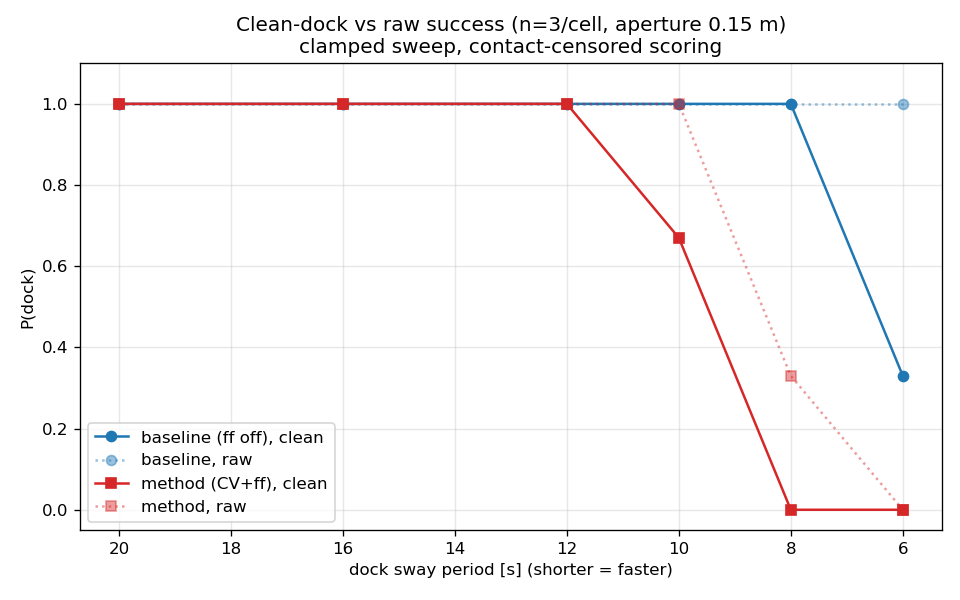
\includegraphics[width=0.8\textwidth]{Figures/clean_pdock.png}
    \caption{Docking success versus sway period under raw (dotted) and
    contact-censored clean (solid) scoring.}
    \label{fig:pdock}
\end{figure}

Clean insertions cross the entry plane 0.003 to 0.05~m off axis at 0.06 to
0.11~m/s closing speed, and all observed contacts occur below 0.06~m/s.
These figures form the interface requirement for a capture mechanism: a
funnel with a capture radius of at least 0.15~m and tolerance for
approximately 0.1~m/s closing speed captures everything the baseline
delivers down to 8~s periods.

\subsubsection{Failure analysis: ego-motion instability of the velocity
estimator}

The method's fast-period failures trace to a single mechanism. The dock
measurement is reconstructed in the world frame through the transform of a
moving camera, so a fraction of the vehicle's own motion leaks into the
measured dock position. This leakage is \emph{correlated with the vehicle
state}, violating the filter's white-noise assumption. The static filter,
with no velocity state, absorbs it as position noise and remains faithful
(estimated sway amplitude 0.7 to 0.9 times truth in all baseline runs). The
constant-velocity filter integrates it into a phantom dock velocity and
extrapolates: estimated amplitude reaches 2.4 to 5 times truth in
successful method runs and 18 to 52 times truth in the failures, where the
estimate has decoupled from the real dock (correlation 0.00 with the true
dock while the estimate's excess motion correlates at 0.88 with the
vehicle's own position). The feedforward closes the loop by injecting the
phantom velocity directly into the command; with the identified plant lag
of approximately 240~ms, the loop gain crosses unity between the 10~s and
8~s periods, which is where the measured cliff sits.

The failure is self-concealing: every alignment signal the system exposes
is computed against its own estimate, and in the failed trials those
signals read seat-tolerance alignment (lateral errors of 0.000 to 0.017~m)
while ground truth shows the vehicle 0.17 to 0.48~m off axis at the dock
plane. Only the ground-truth channel exposes the divergence, an argument
for independent verification in any real deployment.

Three progressively stronger mitigations were evaluated. Bounding the
velocity state at the physical dock speed and adding the covariance
ceiling eliminated the metre-scale runaway and the resulting collisions,
but did not restore fast-period docking. Sweeping the process noise
density $\sigma_a$ over 0.02 to 0.16~m/s$^2$ found no stable setting:
estimated amplitude remained 5 to 37 times truth at every value with no
monotonic trend, because a smaller gain also makes the filter slower to
shed an acquired phantom velocity. The baseline's immunity is structural
rather than a tuning point: its velocity gain is exactly zero, and no
finite gain interpolates to that property while the measurement error
remains correlated with vehicle motion. The conclusion is that dock
velocity feedforward from a world-frame constant-velocity estimator
requires explicit ego-motion compensation, by fusing vehicle odometry into
the filter or estimating in a vehicle-relative frame, identified as future
work.

\subsubsection{Replication}

The sweep was run in full on two hosts (real-time factors 0.6 and 1.0) and
two filter revisions (before and after the velocity bounds). The
baseline's uniform success and the method's cliff between 10~s and 8~s
reproduced in both, indicating the result reflects the estimator design
rather than compute load, hardware or incidental tuning.

\subsection{Part B: Real-CV results}
\label{sec:results-b}

\subsubsection{Detection rate versus marker size and range}

Detection is governed by apparent size in pixels with a sharp floor.
Across all four size groups the rate is zero below 21~px, transitional in
the 21 to 28~px bin (0.21 to 0.59 depending on size), and above 0.85 from
38~px upward (Figure~\ref{fig:det-px}). On the derived metric axis this
maps to overall on-axis rates of 0.93 for the 149.4~mm markers, 0.61 at
74.7~mm, 0.43 at 44.4~mm and 0.29 at 35.6~mm over the swept range. The
oblique run (median incidence 58$^\circ$) detected only the 149.4~mm
markers, at 0.60 overall; the three smaller groups produced zero
detections in 791 trials, indicating that oblique viewing costs roughly
one size class even before the angle reaches the detector's geometric
limits.

\begin{figure}[H]
    \centering
    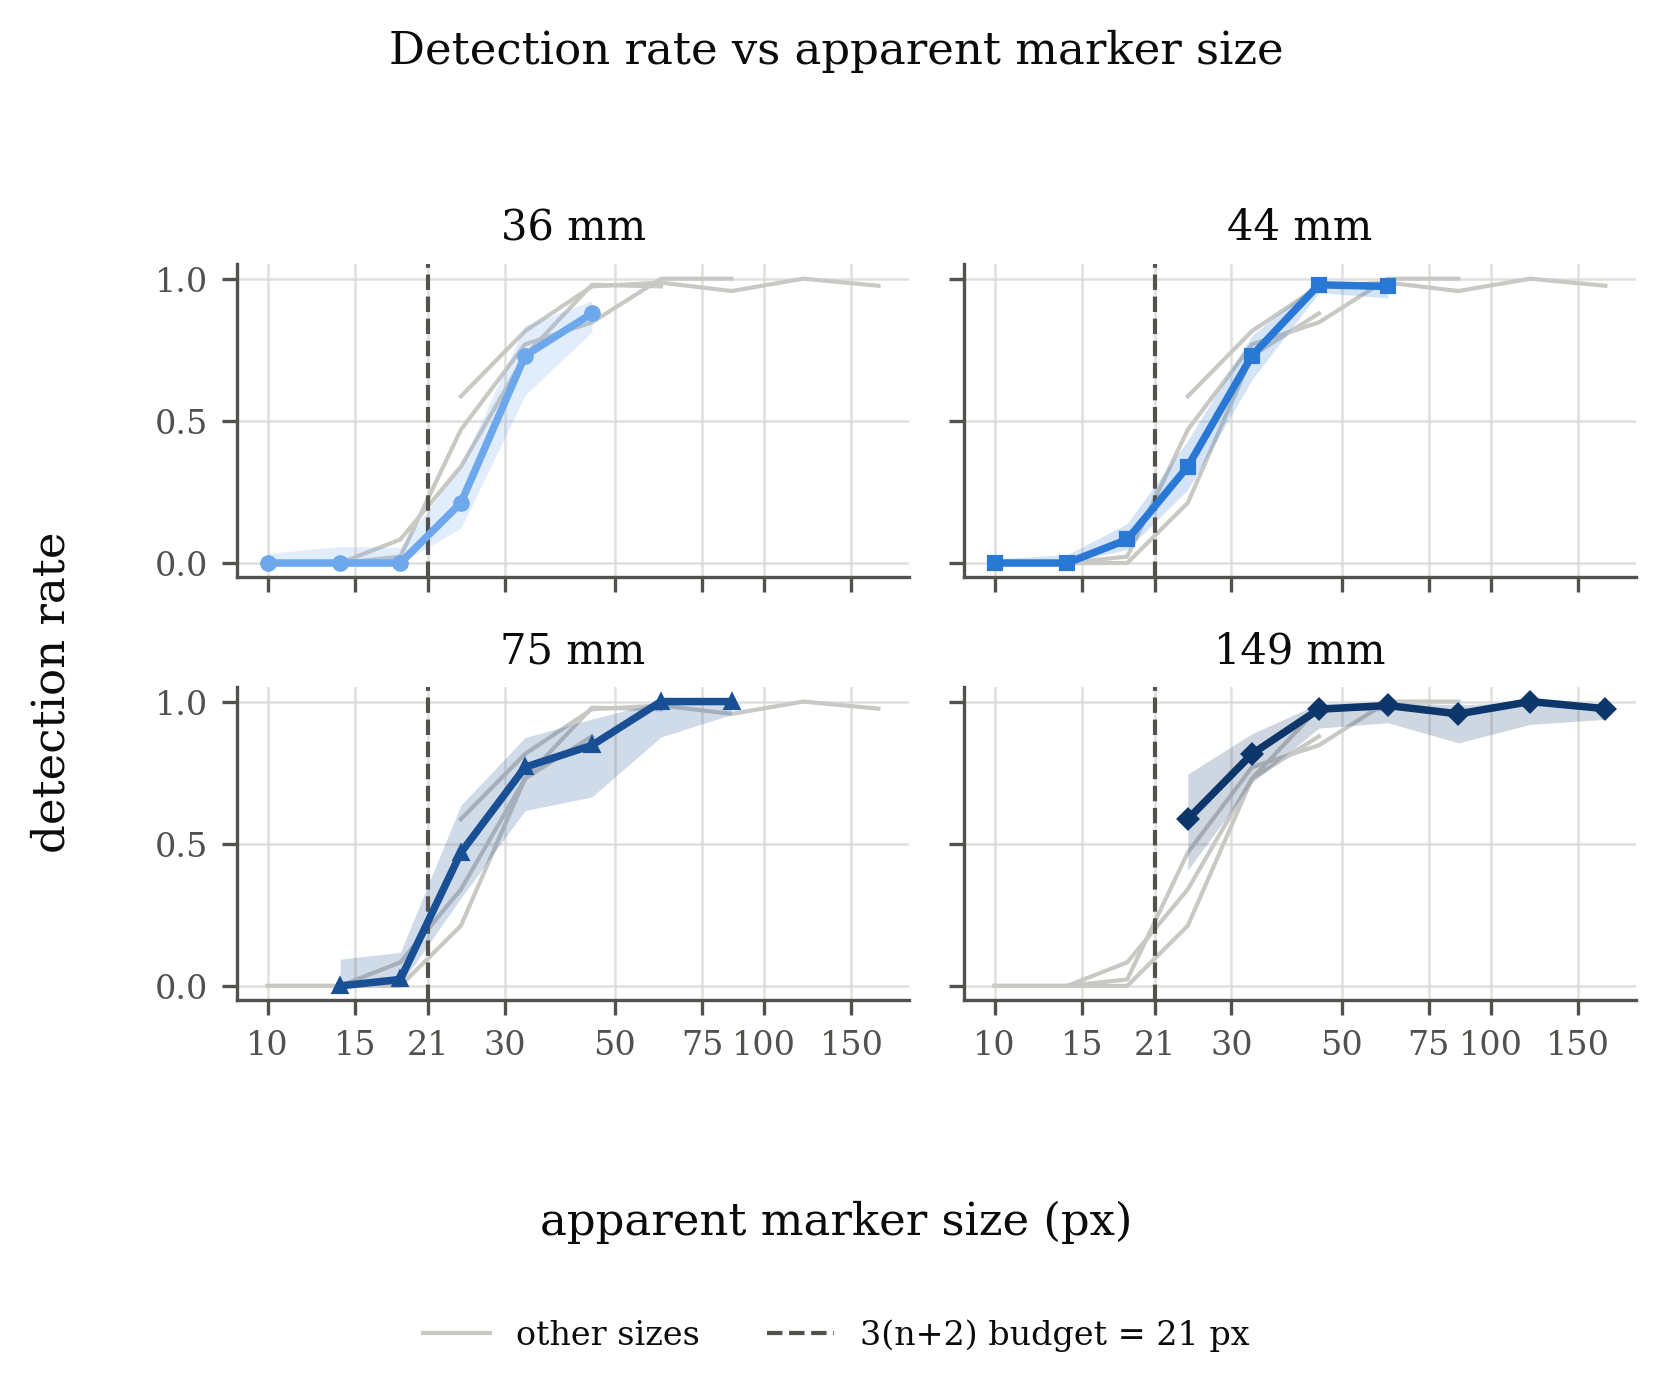
\includegraphics[width=0.95\textwidth]{Figures/detection_rate_vs_px.png}
    \caption{Detection rate versus apparent marker size (pixels), per
    marker size group, with Wilson 95\% intervals; bins with fewer than
    ten trials suppressed. The axis is calibration-free.}
    \label{fig:det-px}
\end{figure}

\subsubsection{Maximum detection range}

Uncensored maximum detection ranges scale linearly with marker side: 5.10
and 4.87~m for the two 149.4~mm markers, 3.05~m at 74.7~mm, 1.55 to
2.17~m at 44.4~mm, and 1.10 to 1.14~m at 35.6~mm, fitted by
$\mathrm{max\ range} \approx 34.9 \times \mathrm{side}$
(Figure~\ref{fig:max-range}). The walk-back continued approximately 3~m
past the last detection with none recorded, so these are genuine detection
limits. Two distinctions matter operationally. First, only the largest
markers reach the 5~m acquisition range assumed for the coarse phase, and
only marginally. Second, maximum range is a single-tail-detection
statistic; the \emph{reliable} (50\%) range sits lower, at 5~m a 149.4~mm
marker subtends 23.8~px, below the $\sim$27~px needed for 50\% detection
(Section~\ref{sec:results-turbidity}), which is why its maximum range of
5.1~m coexists with a 50\% range nearer 4.3~m. Only the second number
sizes a dock.

\begin{figure}[H]
    \centering
    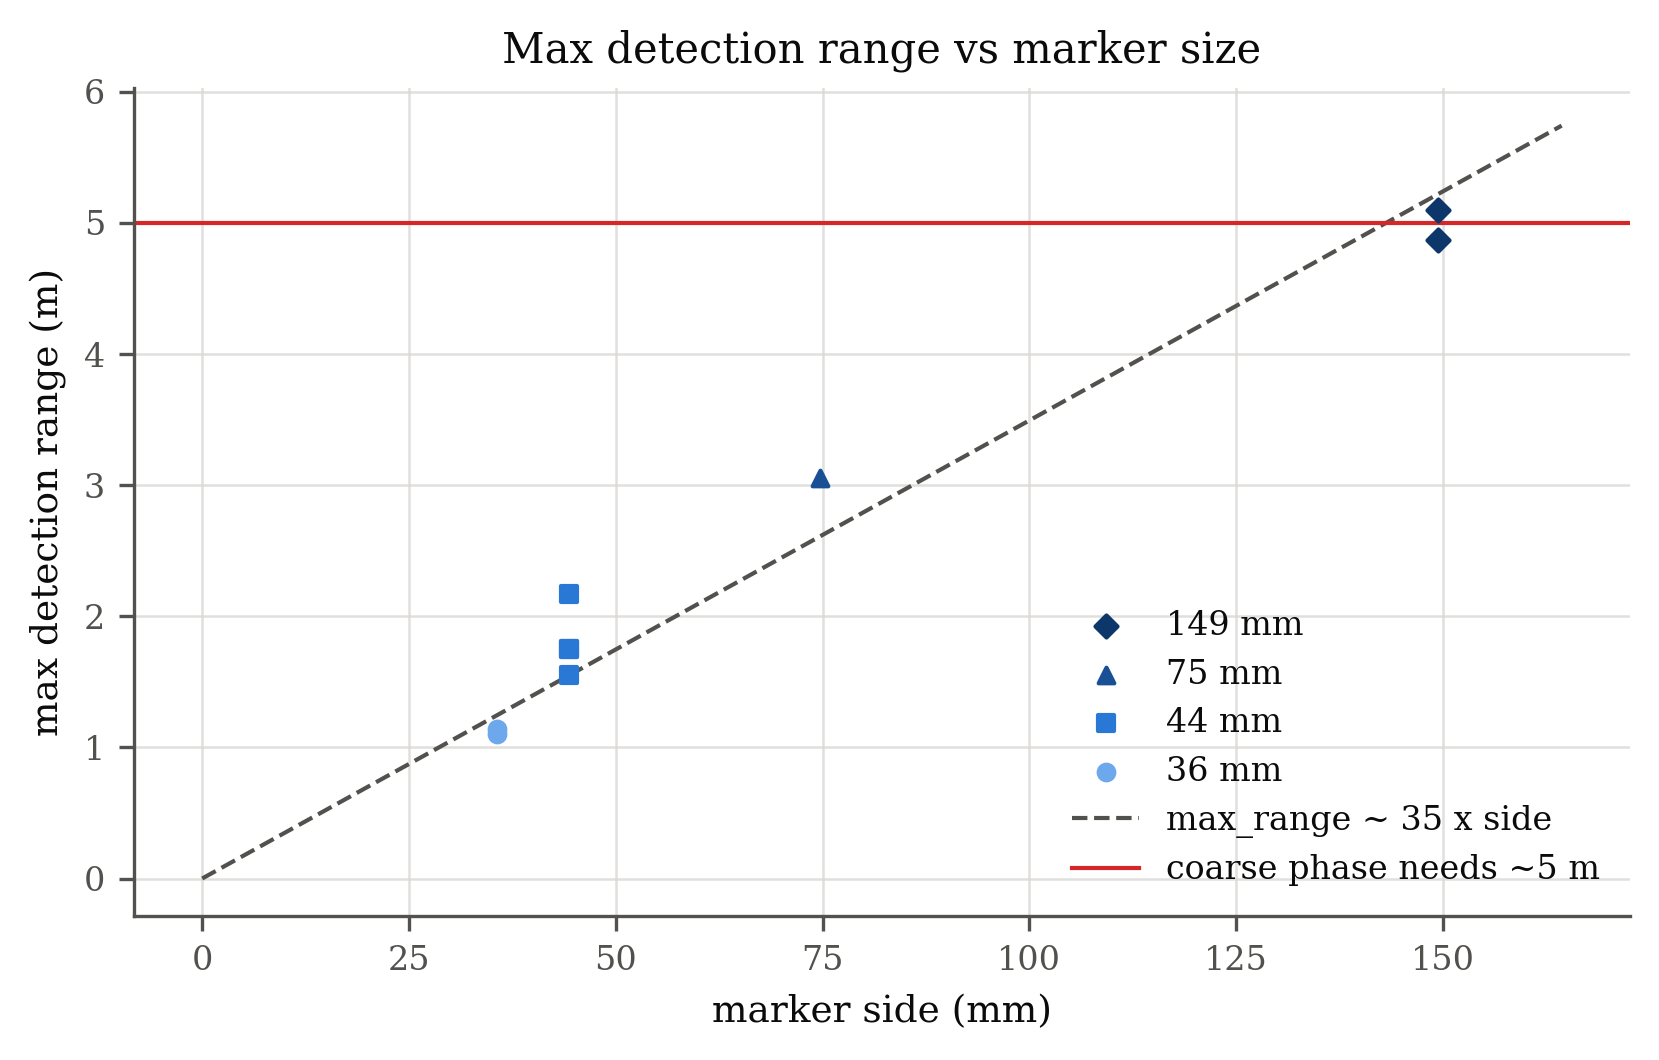
\includegraphics[width=0.8\textwidth]{Figures/max_range_vs_size.png}
    \caption{Maximum detection range versus marker side with the fitted
    linear law and the 5~m coarse-acquisition reference line.}
    \label{fig:max-range}
\end{figure}

\subsubsection{Pose self-consistency and misidentification}

With no external ground truth, single-marker pose is scored against a
leave-one-out multi-marker board reference, a self-consistency measure,
not accuracy. Translation deviation grows from 10.6~mm mean (9.4~mm
jitter) in the 0.5 to 1.0~m bin to 36.1~mm mean (32.9~mm jitter) at 2.0
to 3.0~m; rotation deviation is 11 to 16$^\circ$ and roughly flat with
range. These figures pool all marker sizes, since a per-size split would
change the reference geometry with the marker under test and read
backwards. The sole camera-independent validation is an IMU gravity
check: over 323 frames the board's estimated tilt from vertical has a
median of 6.6$^\circ$, consistent with a hand-held, approximately
vertical board. A yaw-rate cross-check was not corroborative (only 7 of
25 turn segments had sufficient board coverage, and vision magnitudes did
not track the gyro), and is reported as such. Misidentification was
essentially absent in real water: one off-board ID in 1376 on-axis
detections (rate 0.0015) and none in the oblique run.

\subsubsection{Attenuation measurement}

The B-free contrast fit yields, with instrument correction and per-marker
intercepts over 934 samples spanning 0.62 to 3.19~m: $\beta_b = 0.279$,
$\beta_g = 0.247$, $\beta_r = 0.443$, $\beta_{grey} = 0.289$~m$^{-1}$
($r^2 = 0.71$, 0.67, 0.88, 0.75; Figure~\ref{fig:beta}). The strongest
support for the correction chain is a quantity it never saw: the
red-to-green attenuation ratio moves from 1.50 (raw) to 1.79 (corrected),
against approximately 1.8 expected from water optics. A residual check
over 5629 near-to-far marker pairs (not a statistical cross-validation,
no holdout was used) shows the exponential form predicts real far-frame
contrast to a median error of $-3.1$\% corrected, versus $+18.5$\% raw.
At 5~m this water gives a grey optical depth $\tau = 1.44$, i.e.\ 23.6\%
of contrast surviving. The fitted veiling light $B$ is explicitly not
physically meaningful (negative $r^2$; the green estimate exceeds the
white sheet's own brightness): the method is built so that $B$ cancels
from contrast, and $B$ enters the synthesis only as a DC term that
adaptive thresholding rejects.

\begin{figure}[H]
    \centering
    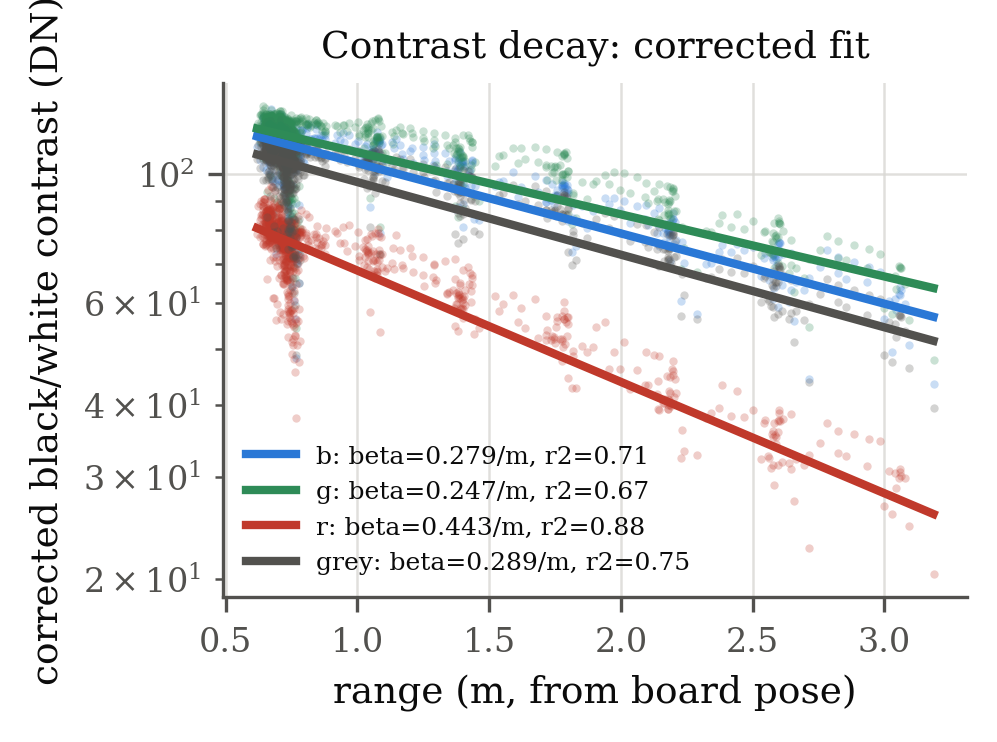
\includegraphics[width=0.8\textwidth]{Figures/beta_contrast_decay.png}
    \caption{Instrument-corrected black-to-white contrast versus range
    with the fixed-effects exponential fits per channel.}
    \label{fig:beta}
\end{figure}

\subsubsection{Turbidity envelope and marker sizing}
\label{sec:results-turbidity}

Re-attenuating all 2551 on-axis trials at ten turbidity multipliers (a
fixed denominator at every level) maps the detection envelope over
apparent size and total optical depth (Figure~\ref{fig:surface}). The
envelope has two regimes: below $\tau \approx 2$ the boundary is
vertical, detection is \emph{pixel-limited} and turbidity hardly moves
it; above $\tau \approx 2.3$ the boundary is horizontal, detection
collapses at every apparent size sampled, \emph{turbidity-limited}. The
pixel budget quantifies the first regime: the apparent size needed for
50\% detection is 27.3 to 28.1~px, flat across a sevenfold span of
optical depth ($\tau$ 0.18 to 1.30), rising only within the resolution of
the binning before the collapse (Figure~\ref{fig:pxbudget}). Two
conclusions follow: the textbook budget of $3(n{+}2) = 21$~px for a
5$\times$5 marker underestimates the real requirement by about 30\%,
because it is a pure sampling argument that assumes air; and ArUco's
adaptive thresholding makes detection remarkably insensitive to contrast
loss until an abrupt threshold near $\tau \approx 2$, a cliff, not a
gradient.

\begin{figure}[H]
    \centering
    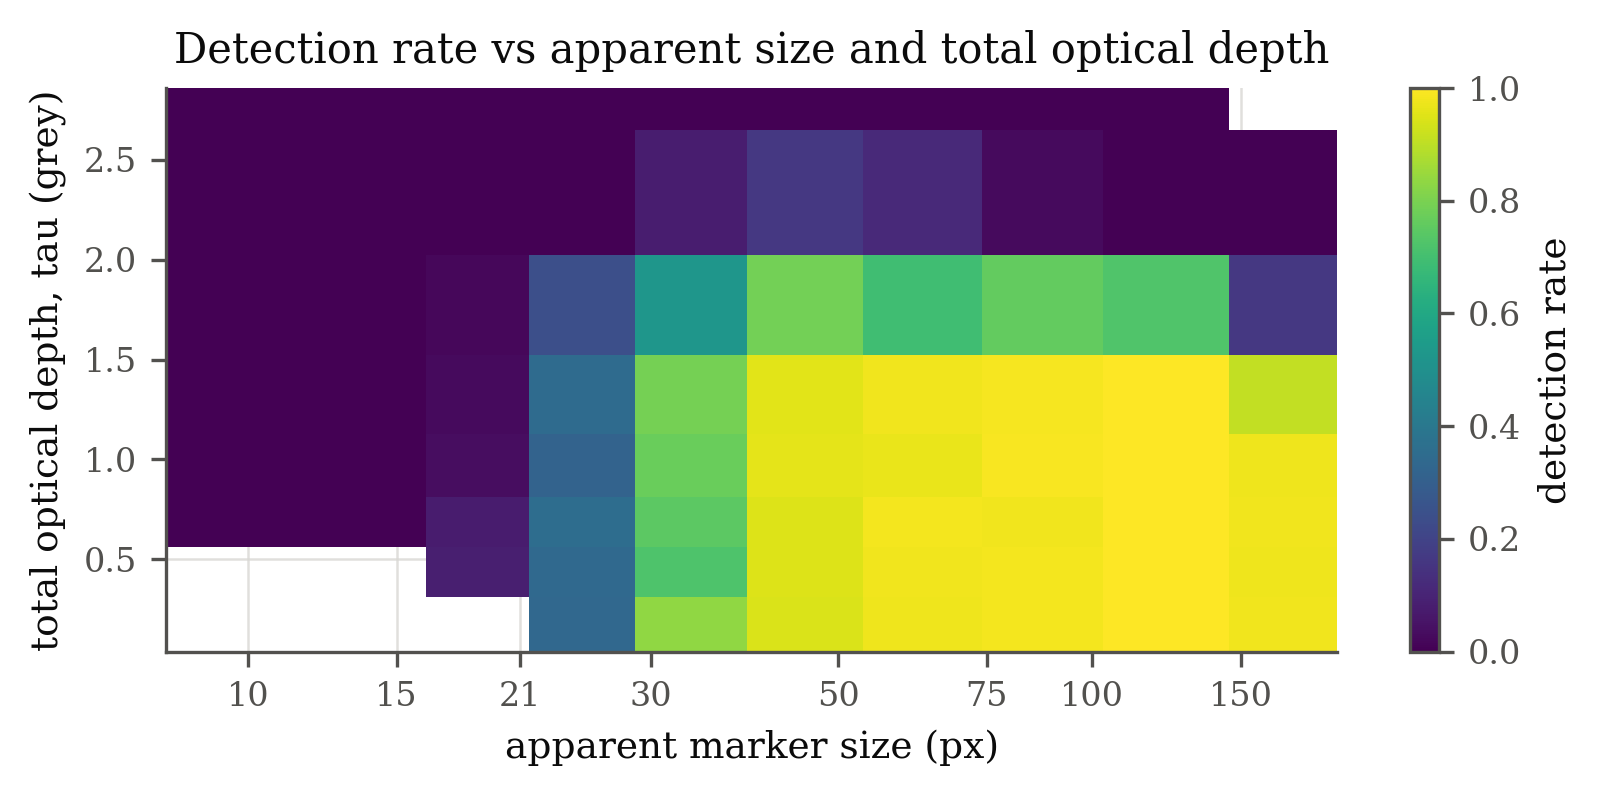
\includegraphics[width=0.9\textwidth]{Figures/rate_px_tau_surface.png}
    \caption{Detection rate over apparent size and total optical depth.
    The boundary is vertical (pixel-limited) below $\tau \approx 2$ and
    horizontal (turbidity-limited) above. White cells are physically
    unreachable combinations.}
    \label{fig:surface}
\end{figure}

\begin{figure}[H]
    \centering
    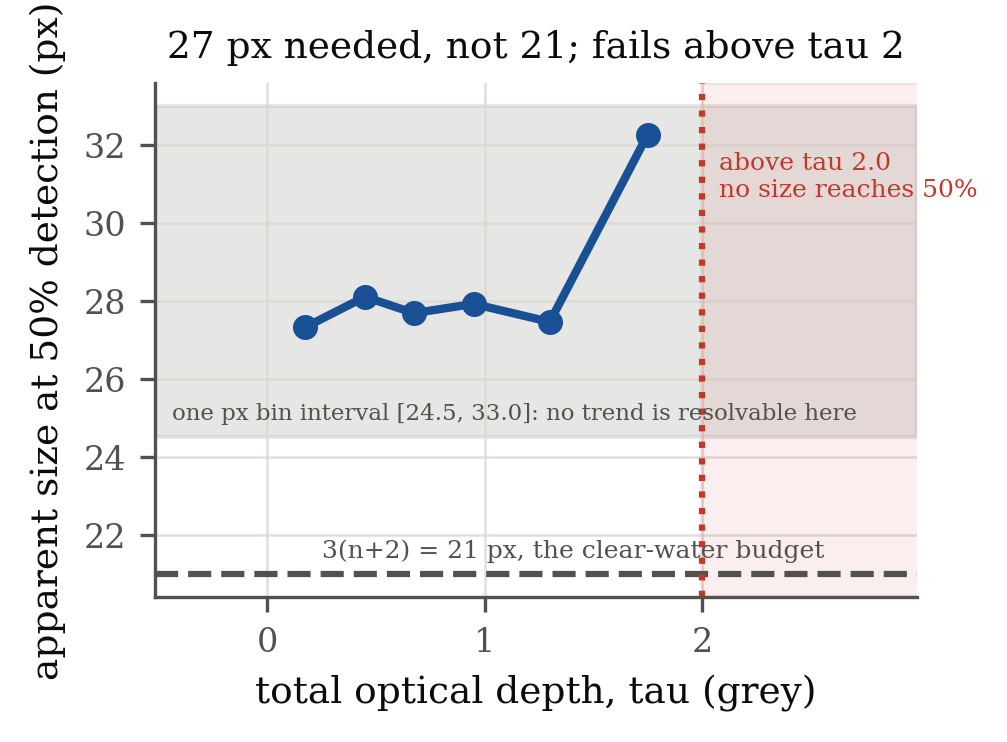
\includegraphics[width=0.8\textwidth]{Figures/px_required_vs_tau.png}
    \caption{Apparent size required for 50\% detection versus optical
    depth: flat at $\sim$27~px across $\tau$ 0.18 to 1.30 (band shows the
    bin-interpolation resolution), undefined above $\tau \approx 2$ where
    no size sampled reaches 50\%.}
    \label{fig:pxbudget}
\end{figure}

Inverting the pixel budget through the pinhole model sizes the dock
marker: for 50\% single-frame detection this pool's water requires a
105~mm marker at 3~m and 182~mm (interval 154 to 207~mm) at 5~m. In
clearer water ($\beta = 0.15$~m$^{-1}$) the 5~m requirement barely drops
(174~mm), confirming that below the cliff the requirement is set by
pixels, not water; in murkier water ($\beta \geq 0.6$~m$^{-1}$, $\tau
\geq 1.8$ at 3~m) the requirement is undefined within the measured
envelope, no marker size sampled achieves 50\%. The textbook 21~px budget
would have specified 132~mm at 5~m, 38\% short in side length and roughly
half the area. The synthesised degradation is illustrated in
Figure~\ref{fig:strip}; a forward-scatter check found no measurable edge
blurring within apparent-size bins across the synthesised range
(slopes scatter around zero), so at these optical depths contrast loss,
not blur, is the operative mechanism.

\begin{figure}[H]
    \centering
    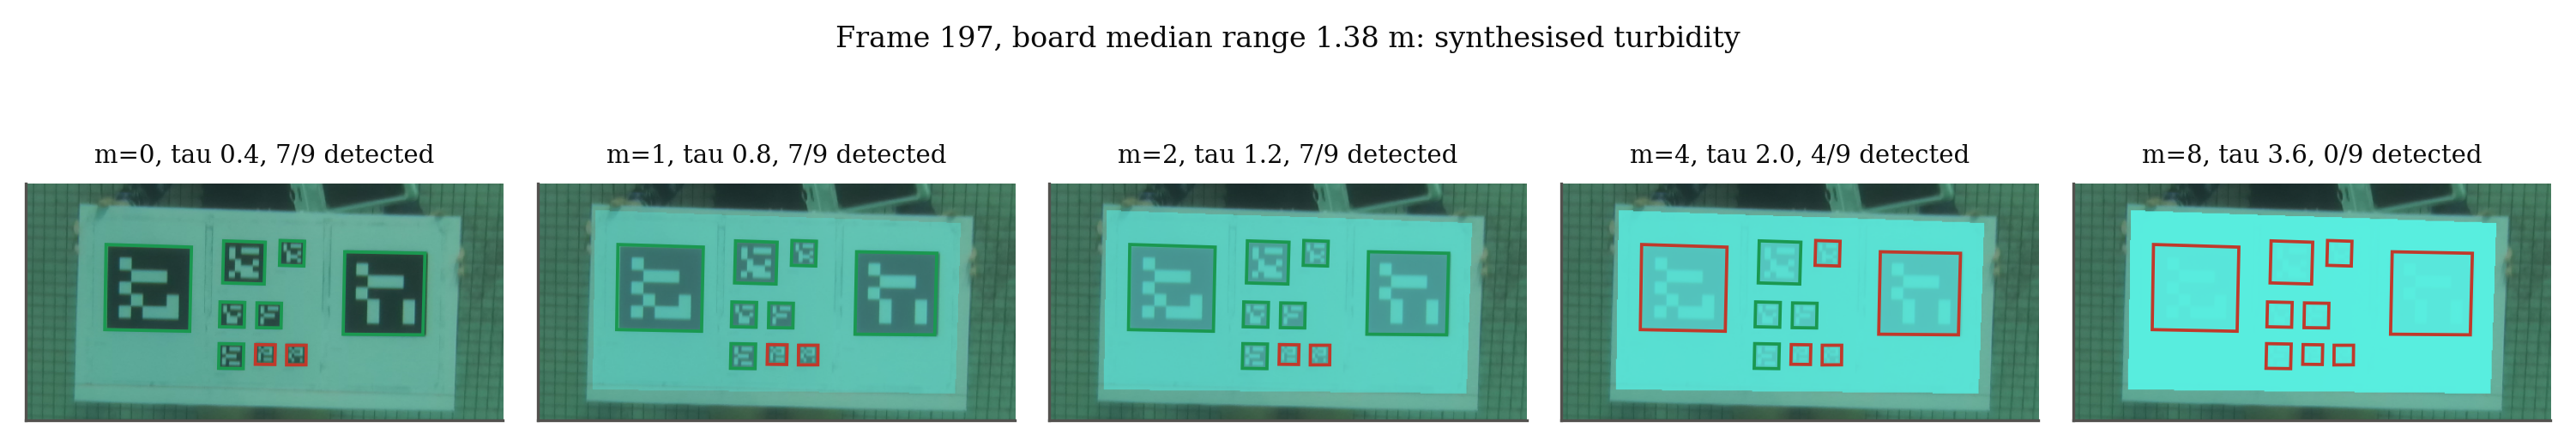
\includegraphics[width=0.95\textwidth]{Figures/synthesis_sweep_strip.png}
    \caption{One frame re-attenuated at increasing turbidity multipliers
    with detections outlined: 7 of 9 markers at the real condition
    falling to 0 of 9 at the highest multiplier. The highest-multiplier
    panel is a diagnostic of the synthesis (its DC term is unphysical),
    not a depiction of real murky water.}
    \label{fig:strip}
\end{figure}

\subsubsection{Preprocessing: CLAHE evaluated and rejected}

CLAHE was evaluated against the detector's own thresholding knob over all
2551 trials at every turbidity level. In \emph{real} water (multiplier 0)
CLAHE is a net negative: detection 0.512 versus 0.519 baseline, while
introducing 0.022 misidentifications per frame where the baseline has
zero. Its apparent gain at high synthesised turbidity (0.337 versus 0.159
at the highest level) is measured on frames whose degradation adds no
scattering noise, and is therefore an upper bound unproven for real
water. Lowering \texttt{adaptiveThreshConstant} to 3 recovers about
two-thirds of that gap (0.276) at a third of CLAHE's misidentification
rate (Figure~\ref{fig:preproc}). The engineering decision follows the
real-water evidence: no CLAHE stage in the pipeline; tune the detector's
threshold constant instead.

\begin{figure}[H]
    \centering
    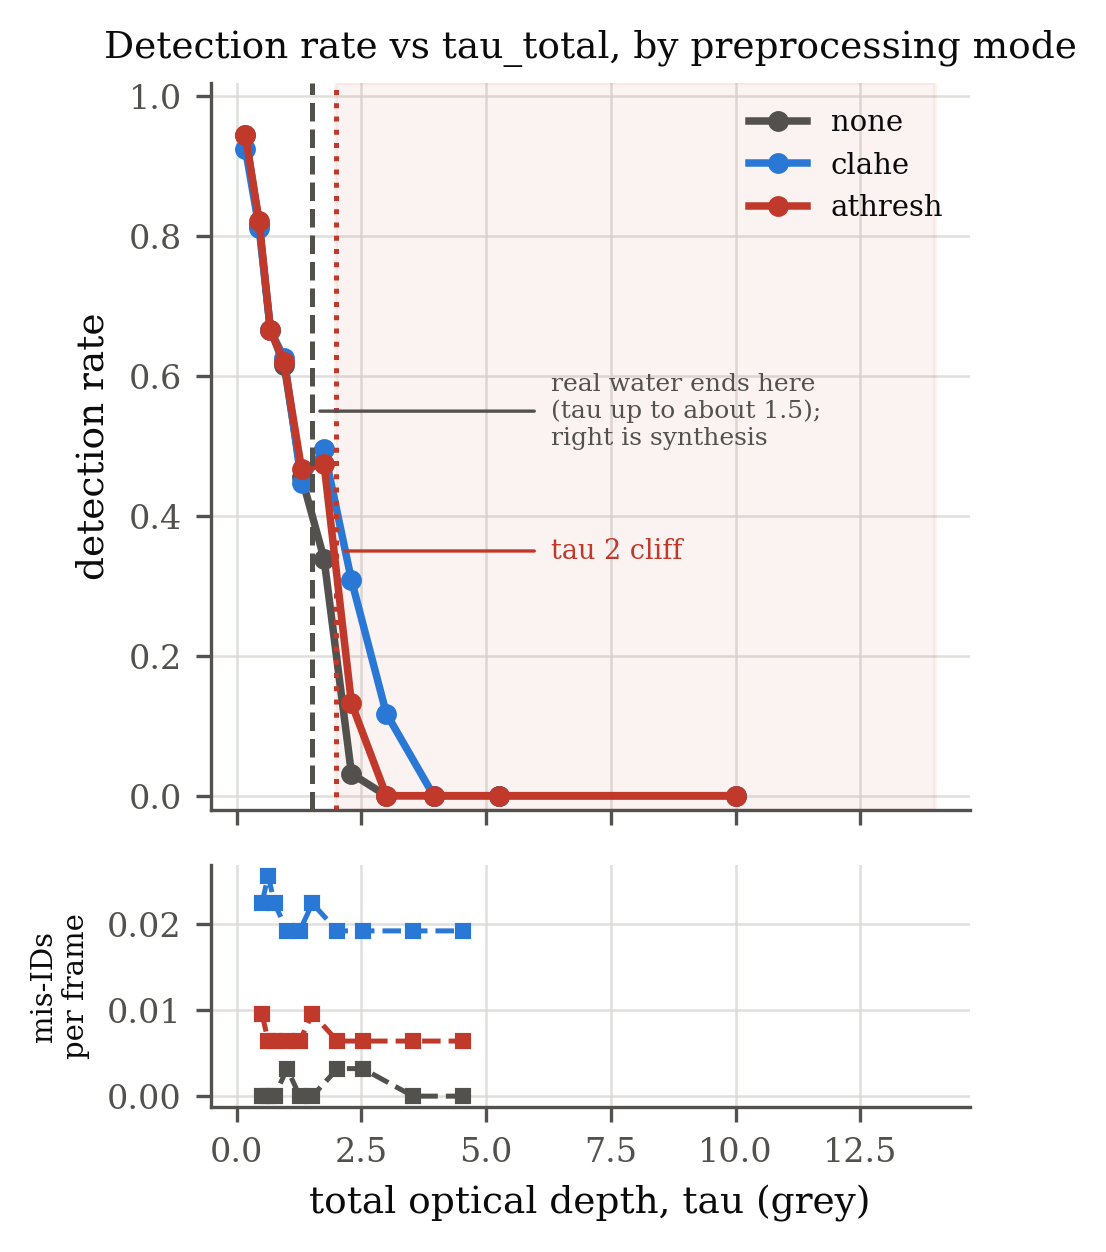
\includegraphics[width=0.9\textwidth]{Figures/preprocessing_eval.png}
    \caption{Detection rate (top) and misidentifications per frame
    (bottom) versus total optical depth for no preprocessing, CLAHE, and
    a lowered adaptive-threshold constant. Real water ends at the dashed
    line; everything beyond is synthesised.}
    \label{fig:preproc}
\end{figure}

\subsubsection{Limitations}

The dataset is one pool, one session: the optical-depth axis is designed
to generalise (results are reported against $\tau = \beta d$), but this
water is a single point and the attenuation spectrum of other waters will
differ. No external ground truth exists; pose results are
self-consistency only, and all metric ranges carry $\pm$10\% from the
in-air focal length. $\beta$ was fitted over 0.62 to 3.19~m, so quoting
$\tau$ at 5~m assumes $\beta$ constant with range. The oblique run is
thin (161 detections, largest markers only) and viewing angle was never
controlled. The capture was hand-held, so motion blur is present and
unmodelled, and synthesised turbidity levels derive from the same frames
and are correlated samples, so the quoted confidence intervals understate
uncertainty at high multipliers.

\subsection{Synthesis}

The two halves bound the operating envelope of passive-marker terminal
docking from opposite sides. Part~A bounds the \emph{dynamics}: with the
full perception pipeline in the loop, the vehicle captures a swaying dock
cleanly down to 8~s periods at 0.1~m amplitude, limited by its own
control bandwidth (240~ms plant lag), and delivers insertions a capture
funnel of 0.15~m radius and 0.1~m/s tolerance can accept. Part~B bounds
the \emph{sensing}: a marker is reliably detectable only above
$\sim$27~px of apparent size and below $\tau \approx 2$ of optical
depth, which in the measured water prices the 5~m acquisition range at a
182~mm marker (154 to 207~mm) and rules out reliable acquisition at that
range in substantially murkier water regardless of size.

The intersection is the design statement for the dock. The 200~mm-class
markers assumed throughout Part~A are validated by Part~B as marginally
sufficient for 5~m acquisition in pool-clarity water, with the
per-size fusion pipeline of Part~A consuming exactly the size-dependent
envelope Part~B measured (small markers taking over as large ones
overflow the field of view at close range, whose 5~cm blackout sets the
seat criterion). Beyond the measured envelope, at longer standoff or
higher turbidity, the passive-marker channel provides no signal, and
terminal docking must be handed a vehicle already inside the envelope by
a far-field cue such as an active light beacon, which is precisely the
acquisition stage this work scoped out and now quantifies the need for.
% TODO expand: one paragraph tying the failure analysis (ego-motion) to the
% deployment recommendation (vehicle-relative estimation), and one on the
% descoped physical docking trials with this envelope as the justification.
